\chapter{Космическая аппаратура “Плазменный кристалл-4”}
\label{cha:ch_3}
Космическая аппаратура “Плазменный~кристалл~-~4“ (КА~“ПК-4“) была введена в эксплуатацию на борту
Международной космической станции (МКС) в июне 2015~года. Установка предназначена для экспериментального
исследования пылевой плазмы в условиях микрогравитации. В отличие от предыдущей космической аппаратуры
“ПК-3” и “ПК-3~Плюс”, где пылевая плазма создавалась в емкостном радиочастотном (ВЧ) газовом разряде,
в КА~“ПК-4“ пылевая плазма создается в однородном положительном столбе газового разряда в режиме
комбинированного постоянного тока, а также в индуктивном ВЧ разряде. Условия микрогравитации оказывают
влияние на создание вытянутых пылевых облаков в однородном положительном столбе, благодаря чему становится возможным
создать в лабораторных условиях небольшое облако пыли со средним размером 1~см \cite{Usachev-Elbrus}.

\section{Экспериментальная установка}
\label{sec:sec_31}
\begin{figure}[t]
  \centering
  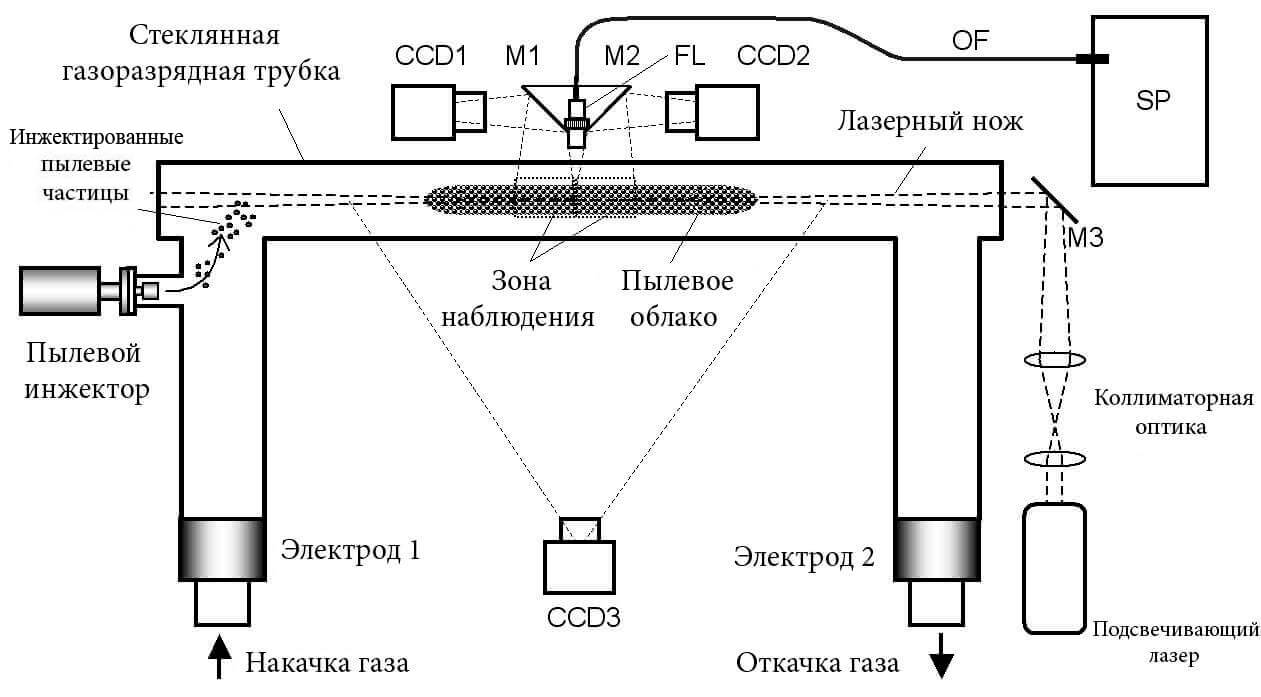
\includegraphics[width=12cm]{figures/fig31}
  \caption{Схема экспериментальной установки космической аппаратуры “Плазменный~кристалл-4”. Здесь CCD1,~CCD2~--~камеры высокого разрешения;
           M1,~M2,~M3~--~зеркала; OF~--~оптоволоконный кабель; SP~--~спектрометр.}
  \label{fig:fig31}
\end{figure}
Основой экспериментальной установки является П-образная стеклянная разрядная трубка с внутренним диаметром 30~мм
и общей длиной 85~см, которая заполнена молекулярным неоном под давлением 60~Па.
На концах трубки установлены цилиндрические электроды из нержавеющей стали, которые используются для создания
и поддержания разряда постоянного тока. Системы вакуумной откачки и накачки газа соединяются с концами трубки
через данные электроды. Прежде, чем трубка заполняется газом, в течение 2~дней она откачивается до давления высокого вакуума порядка \math{< 2 × 10^{-3}}$~Па, а
затем заполняется неоном до рабочего давления разряда порядка 60~Па. Ток разряда составляет \math{I_{DC} = 1}$~мА.

После запонения рабочим газом, с катодной стороны разрядной трубки с помощью пылевого инжектора впрыскиваются
монодисперсные пластические (меламиноформальдегидные) микросферы (частицы пыли) с диаметром \marh{d~=~3.38 ± 0.07}~мкм,
которые, заряжаясь отрицательно, с помощью электрического поля постоянного тока, образуюшегося между катодом и анодом,
транспортируются в центр трубки для дальнейшего наблюдения. Пылевые частицы подсвечиваются зеленым
(532~нм) лазерным «ножом» и регистрируются двумя камерами наблюдения высокого разрешения (CCD1 и CCD2),
а также для наблюдения за подсвеченной плазмой общей камерой наблюдения (CCD3) (см~рис.~\ref{fig:fig31}).

Каждая камера CCD1/CCD2 имеет поле зрения \math{22 × 17}$~мм\math{^2}$, разрешение \math{1600 × 1200}$~пикселей, а также
частоту кадросмен 35~кадров в секунду. Камеры дополняют друг друга, присоединяясь меньшими сторонами и имеют общий размер
\math{44 × 17}$~мм\math{^2}$. Эффективная полуширина лазерного «ножа» составляет 50~мкм в центре поля зрения,
а также 180~мкм по краям.

Камера CCD3 имеет возможность просматривать всю трубку целиком c разрешением \math{640 × 480}$~пикселей
и частотой 15~кадров в секунду. Используя калейдоскопическую систему, камера CCD3 наблюдает плазменное свечение
в центральной части разрядной трубки через 3~спектральных фильтра: один серый фильтр с пропусканием 12\% и два узкополосных
помеховых фильтров, настроенных на 705 и 587~нм.

Одна из копий модифицированной экспериментальной установки КА~“ПК-4“ в собранном виде находится в институте ОИВТ РАН,
которая внешне не имеет существенных отличий (см~рис.~\ref{sub:photo-pk4}).

\begin{figure}[t]
    \begin{center}
         \subfloat[\label{sub:3D-scheme-pk4}]{
           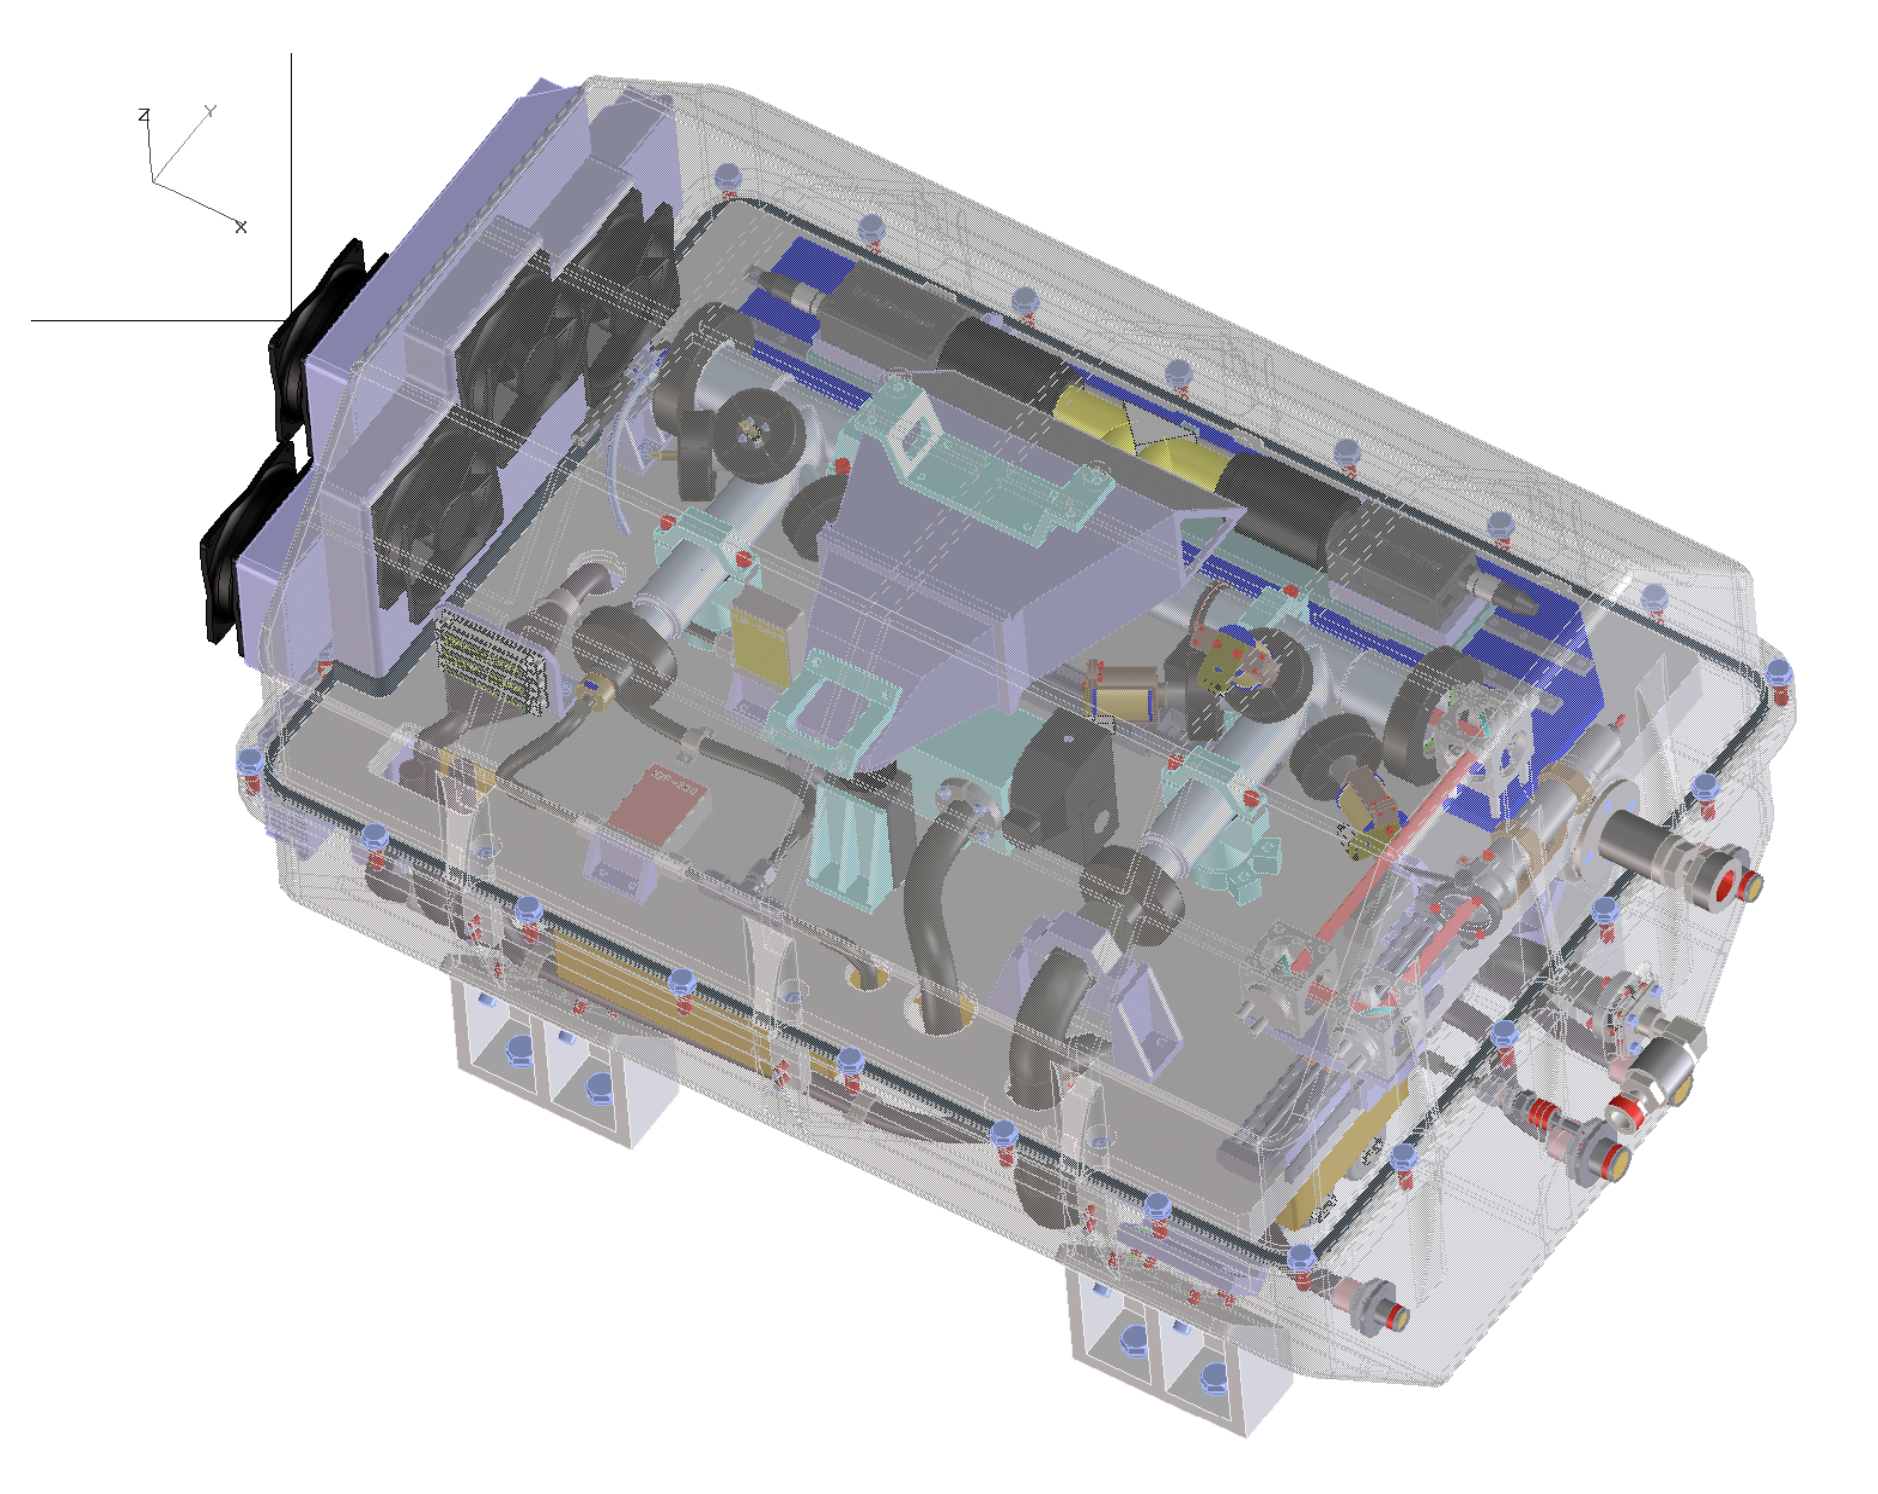
\includegraphics[width=0.35\textwidth]{figures/3D-scheme-pk4}
         }
         \hspace{0.05\columnwidth}
         \subfloat[\label{sub:photo-pk4}]{
           \includegraphics[width=0.35\textwidth]{figures/photo-pk4}
         }
         \caption{Экспериментальная установка космической аппаратуры “Плазменный~кристалл-4”: \pt(a) 3D-модель внутренностей,
                  \pt(b) фото уже собранной установки в лабораторных условиях.}
    \end{center}
    \label{fig:pk4}
\end{figure}

\section{Спектрометр “OceanOptics~USB2000+”}
Для осуществления спектральной диагностики КА~“ПК-4“ применяется модульный мини-спектрометр OceanOptics~USB2000+ (см~рис.~\ref{fig:usb2000+}).
В основе лежит 2048-пиксельная ПЗС-линейка, которая позволяет проводить спектральные измерения в диапазоне длин
волн 350-1100~нм со спектральным разрешением 1.5~нм. Приемная оптика спектрометра устанавливается рядом
с камерами высокого разрешения PO и подключается к спектрометру через оптическое волокно (см~рис.~\ref{fig:fig31}).
Время считывания одного спектра составляет 4~с. Основная цель применения спектрометра в данной аппаратуре - это
контроль чистоты плазмы во время экспериментов на основе спектральных методов поиска примесей.
\begin{figure}[t]
  \centering
  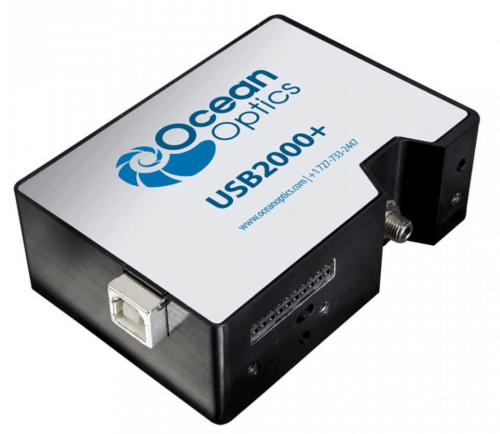
\includegraphics[width=12cm]{figures/usb2000+}
  \caption{Модульный мини-спектрометр OceanOptics~USB2000+.}
  \label{fig:usb2000+}
\end{figure}

\section{Экспериментальные данные}
\label{cha:ch_3_4}
В космической аппаратуре “Плазменный~кристалл-4” выделены следующие каналы получения экспериментальных данных,
которые были задействованы в какой-либо мере в данной работе:
\begin{enumerate}
    \item Видеозаписи с двух камер высокого разрешения CCD1 и CCD2 (см~рис.~\ref{fig:fig32}).
    Видеофайлы в сыром виде имеют формат “.avi” с размером 10~Gb/min.

    \item Видеозаписи с общей камеры наблюдения. Представляют собой файлы в формате … с размером … (см~рис.~\ref{fig:fig33}).
    \begin{figure}[t]
      \centering
      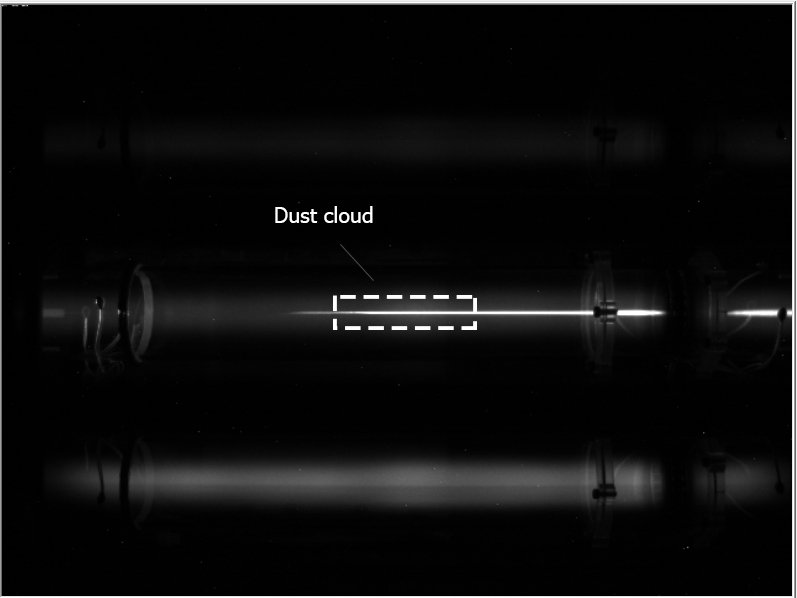
\includegraphics[width=6cm]{figures/fig33}
      \caption{Кадр видеозаписи с общей камеры наблюдения с отмеченным пылевым облаком.}
      \label{fig:fig33}
    \end{figure}

    \item Спектральные данные. Представляют собой текстовые файлы в формате “.dat”,
    которые имеют свою особую структуру, пример можно найти в \hyperref[app:app1]{приложении~А}.


    \item Логи. Представляют собой текстовые файлы в формате “.log”, которые содержат информацию обо всех
    технических изменениях в ходе эксперимента с временными отметками.

    \item В качестве исследования были обработаны сырые спектральные данные, полученные при одних и тех же
    технических условиях системы, в отсутствие пылевого облака, а также в присутствии пылевого облака (см~рис.~\ref{fig:fig34}).
    \begin{figure}
        \centering
        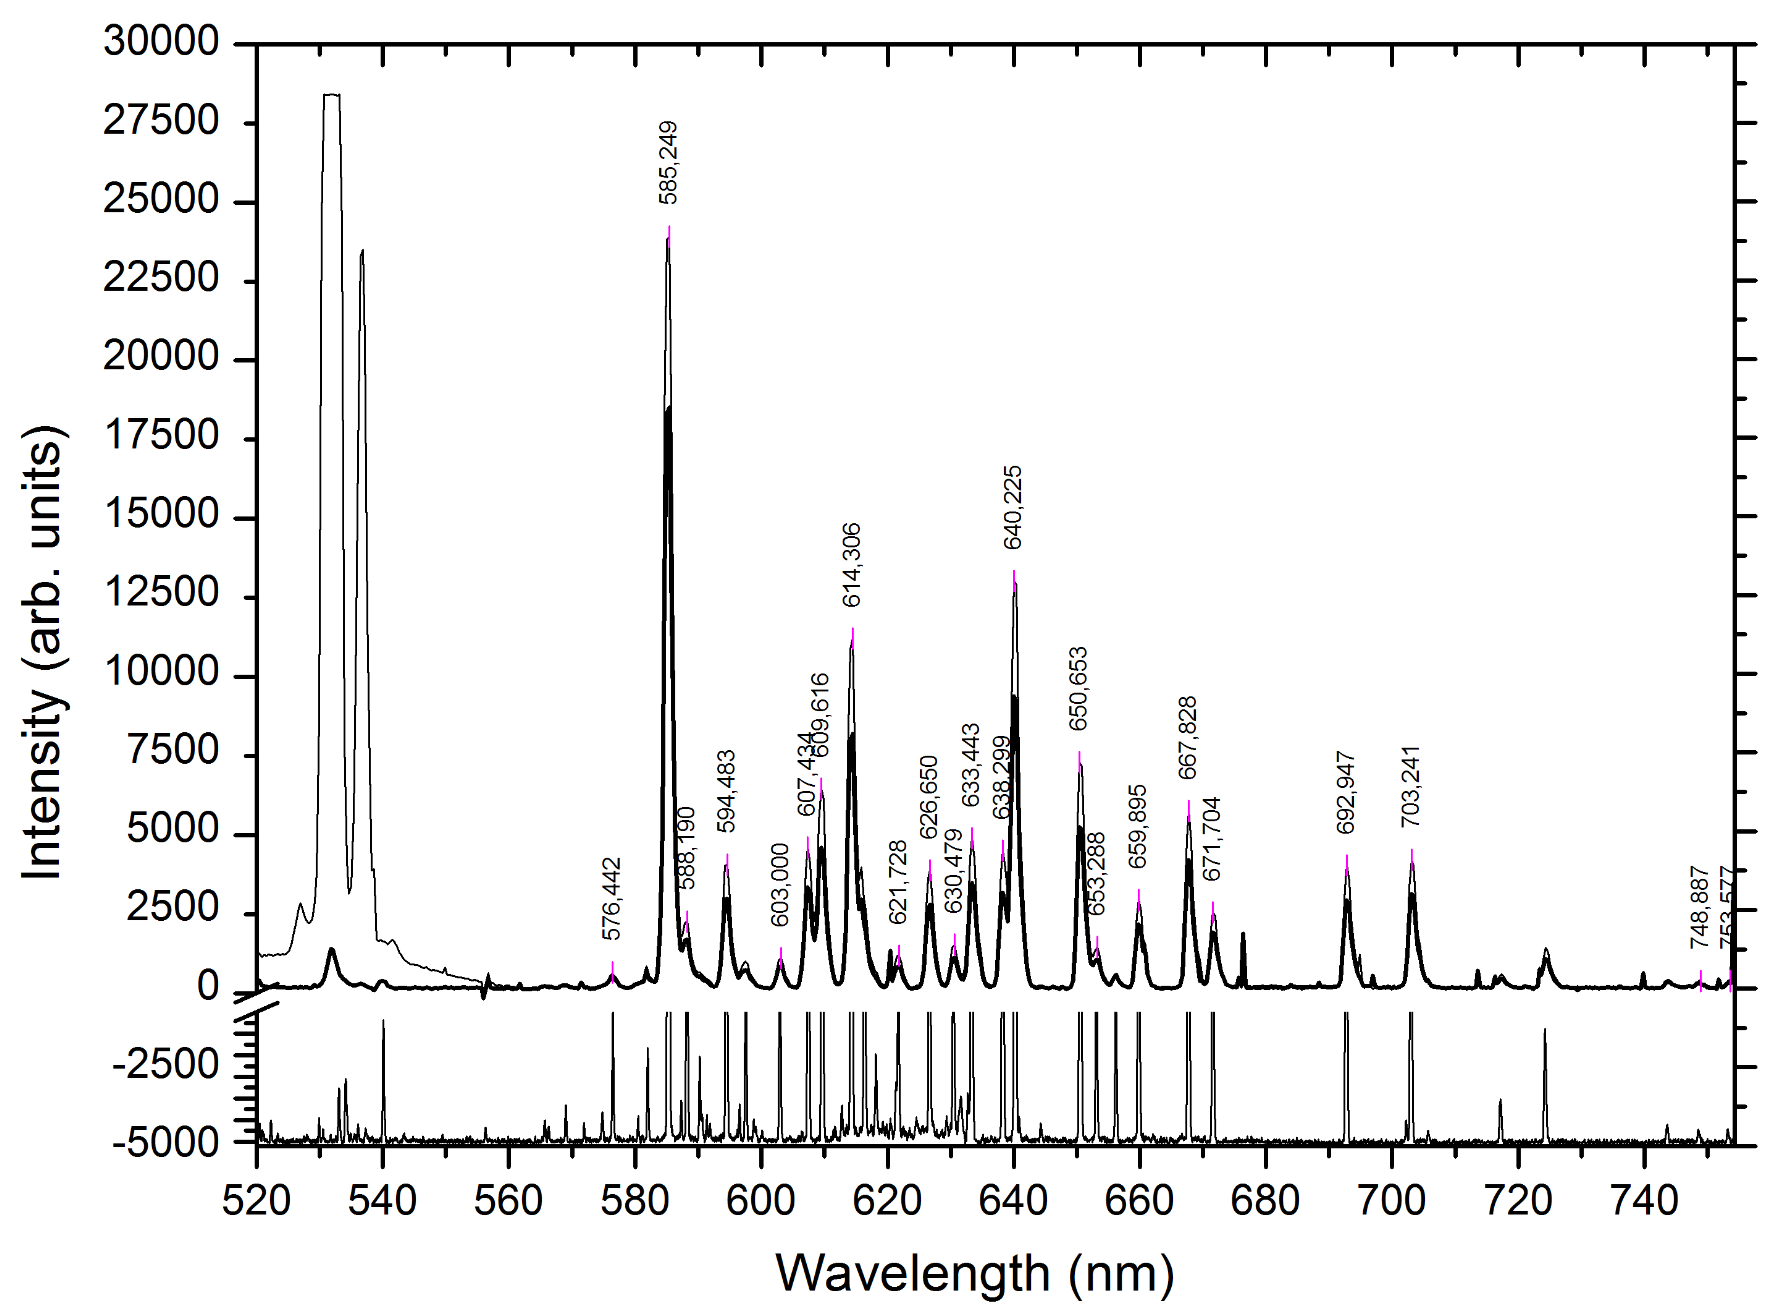
\includegraphics[width=15cm]{figures/fig34}
        \caption{
            Зависимость интенсивности (усл.~ед.) от длины волны (нм). На графике наложены три спектра:
            1. Ниже нуля калибровочный спектр с достоверными линиями неона;
            2. Жирной линией выделен спектр без пылевого облака.
            3. Тонкой линией выделен спектр с пылевым облаком
        }
        \label{fig:fig34}
    \end{figure}
\end{enumerate}

\begin{figure}[t]
  \centering
  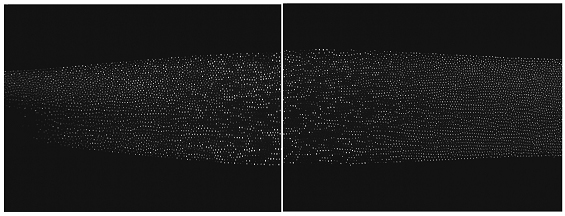
\includegraphics[width=12cm]{figures/fig32}
  \caption{Кадры видеозаписей с двух камер наблюдения высокого разрешения PGO. Кадры синхронизированы во времени, а также пространственно дополняют друг друга.}
  \label{fig:fig32}
\end{figure}


Экспериментально было обнаружено увеличение интенсивности спектральных линий при попадании пылевого облака
в газовый разряд неона, причем линии с разными верхними энергетическими уровнями имеют разные значения
отношений интенсивностей (см~рис.~\ref{fig:fig35}).
\begin{figure}
    \centering
    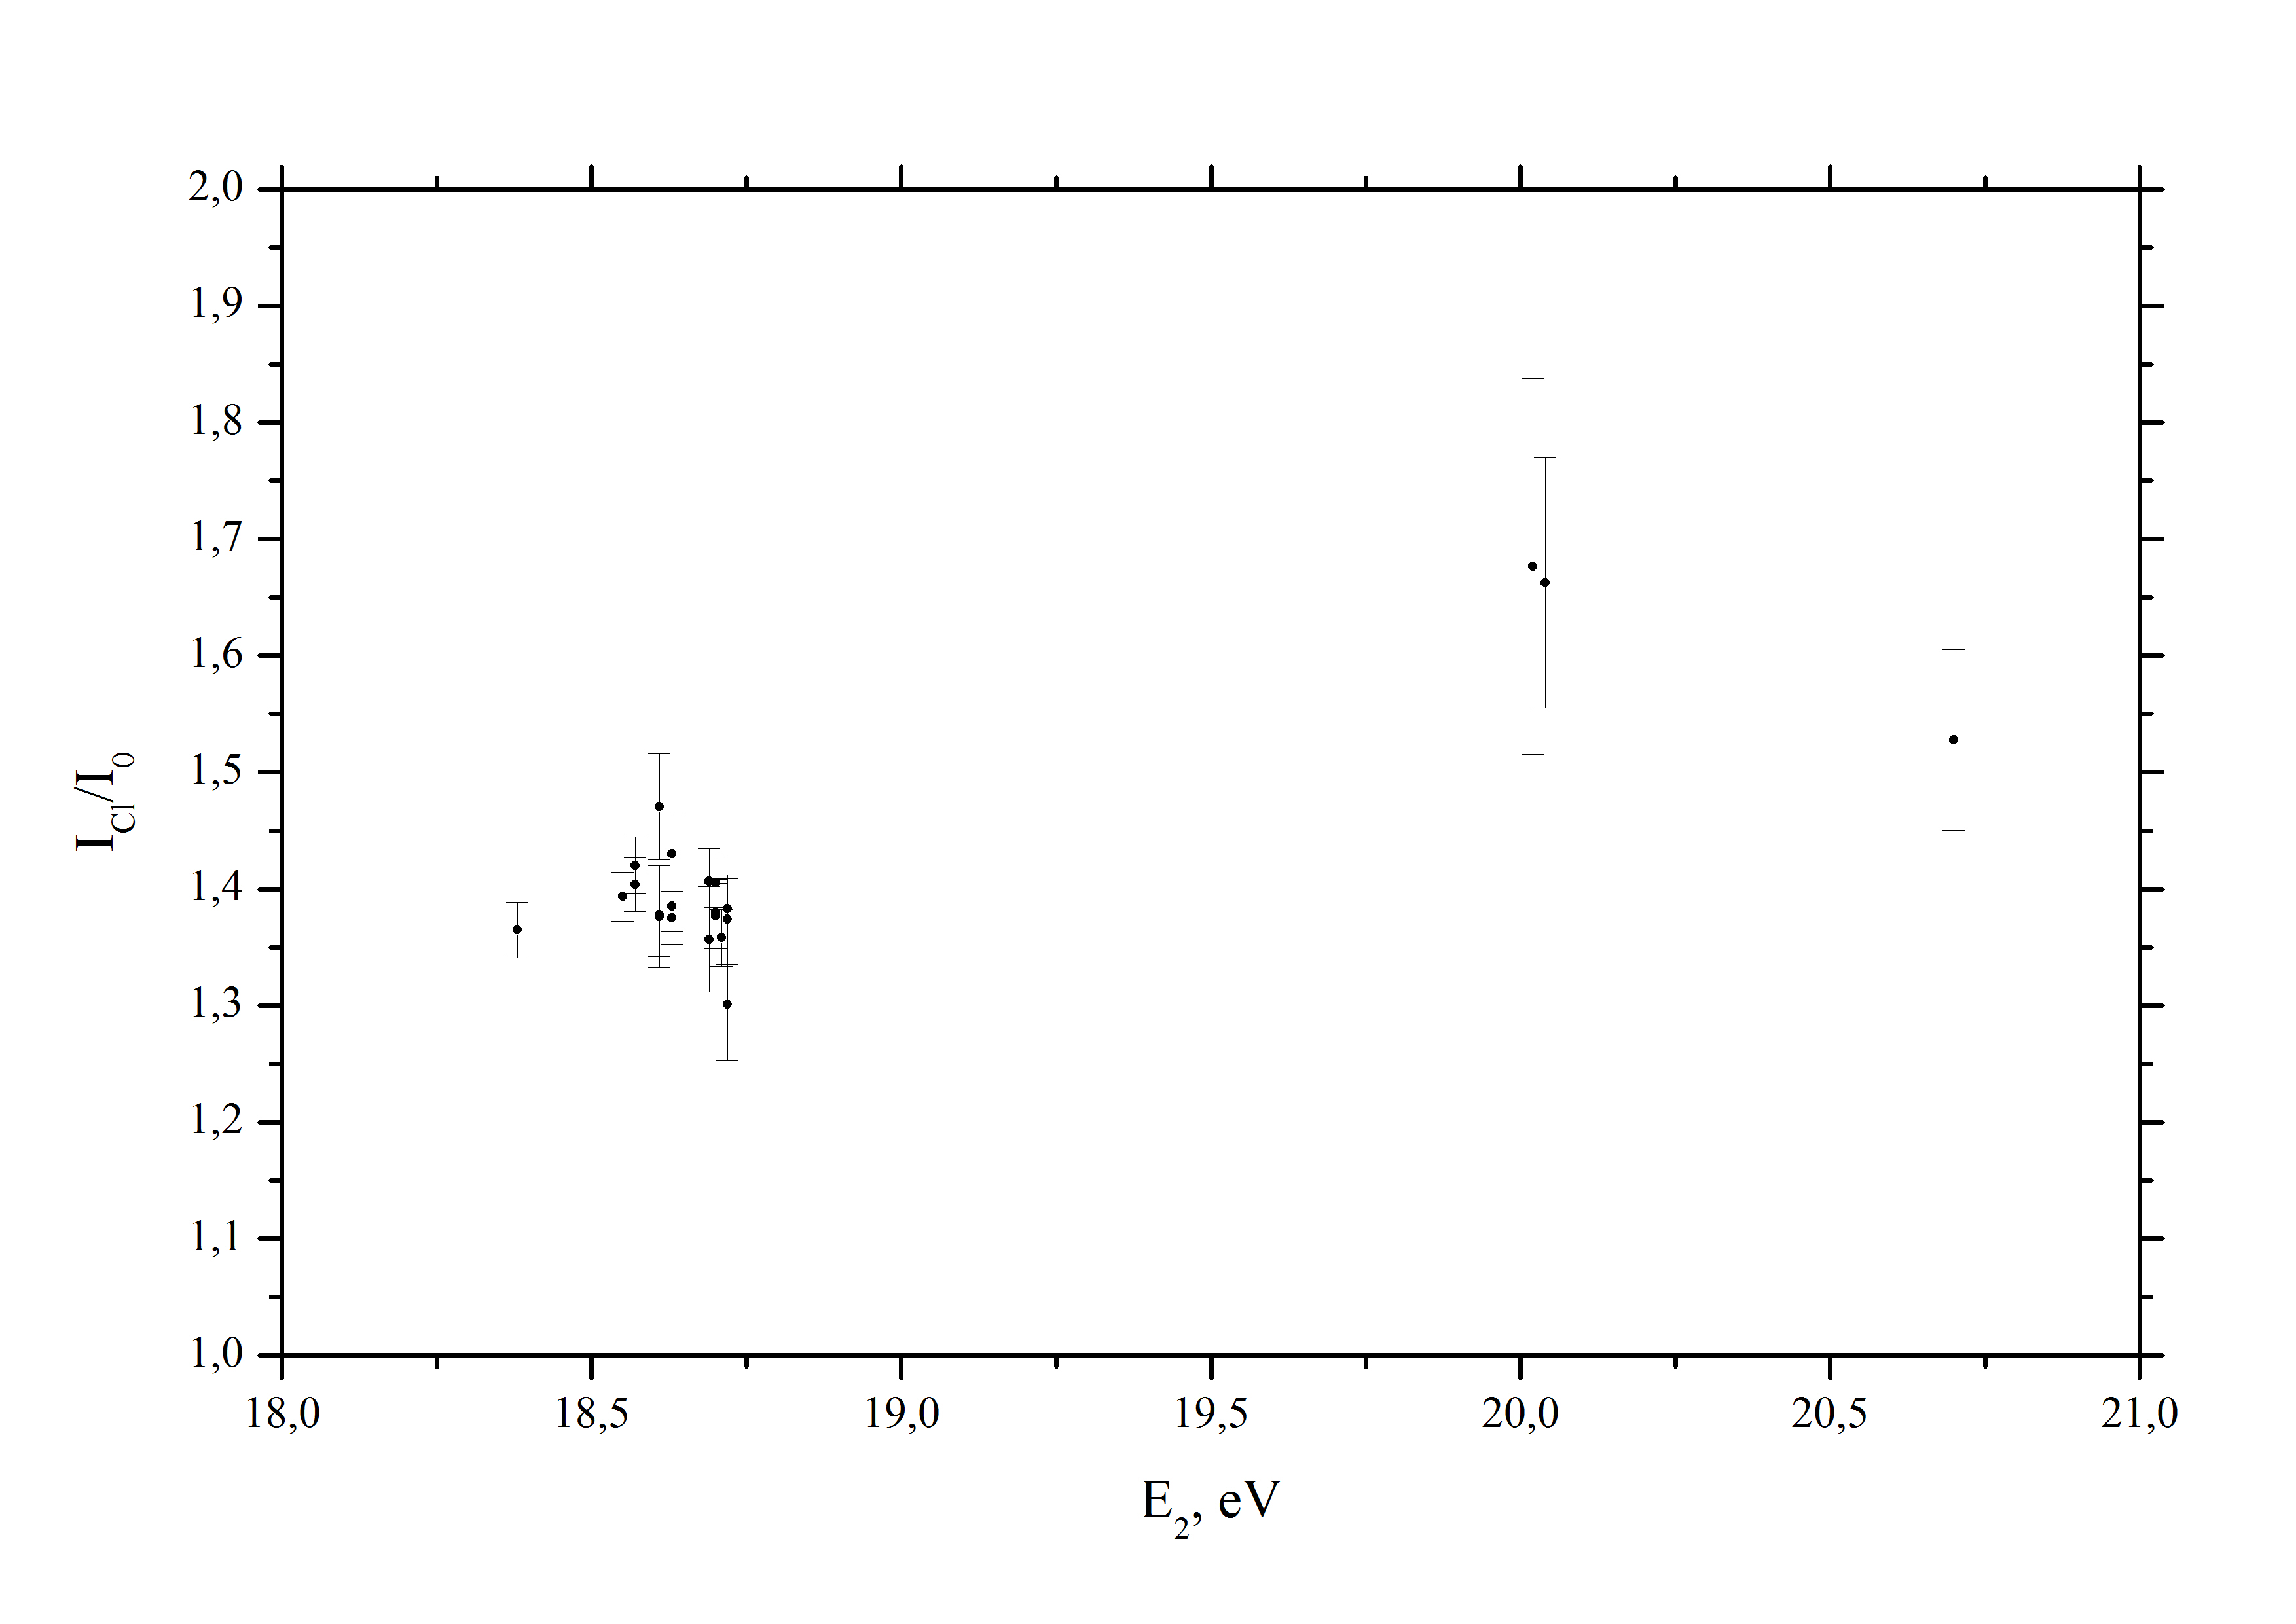
\includegraphics[width=15cm]{figures/fig35}
    \caption{Зависимость отношения интенсивностей спектральных линий неона в присутствии пылевого облака к отсутствию пылевого облака.}
    \label{fig:fig35}
\end{figure}